\documentclass[10pt,a4paper]{article}
\usepackage[right=0.5cm, left=0.5cm,top=1cm,bottom=1.5cm]{geometry}
\usepackage{enumitem}
\usepackage{graphicx}
\usepackage{array, tasks}
\usepackage{blindtext}
\usepackage{fontspec}
\usepackage{amsmath,amsfonts,amssymb,mathrsfs,amsthm}
\usepackage{fancyhdr}
\usepackage{xcolor}
\usepackage{booktabs}
\usepackage[font={bf}]{caption}
% \captionsetup[table]{box=colorbox,boxcolor=orange!20}
\usepackage{float}
\usepackage{esvect}
\usepackage{tabularx}
\usepackage{pifont}
\usepackage{colortbl}
 \usepackage{fancybox}
 \mathversion{bold}
 \usepackage{pgfplots}
 % \usepackage[utf8]{inputenc}
\usepackage{tikz}
 \usepackage[tikz]{bclogo}%
 \usepackage{mathpazo}
\usepackage{ulem}
\usepackage{yagusylo}
\usepackage{textcomp}
\usepackage{blindtext}
\usepackage{multicol}
\usepackage{varwidth}
\usetikzlibrary{calc,intersections}
\usepackage{pgfplots}
%\usepackage{fourier}
\pgfplotsset{compat=1.11}
\usepackage{tkz-tab}
\usepackage{xcolor}
\usepackage{color}
\usetikzlibrary{calc}
\mathchardef\times="2202
\usepackage[most]{tcolorbox}
\definecolor{lightgray}{gray}{0.9}
\definecolor{ocre}{RGB}{0,244,244} 
\definecolor{head}{RGB}{255,211,204}
\definecolor{browndark}{RGB}{105,79,56}
%\RequirePackage[framemethod=default]{mdframed}
\usepackage{tikz}
\usetikzlibrary{calc,patterns,decorations.pathmorphing,arrows.meta,decorations.markings}
\usetikzlibrary{arrows.meta}
\makeatletter
\tcbuselibrary{skins,breakable,xparse}
\tcbset{%
  save height/.code={%
    \tcbset{breakable}%
    \providecommand{#1}{2cm}%
    \def\tcb@split@start{%
      \tcb@breakat@init%
      \tcb@comp@h@page%
      \def\tcb@ch{%
        \tcbset{height=\tcb@h@page}%
        \tcbdimto#1{#1+\tcb@h@page-\tcb@natheight}%
        \immediate\write\@auxout{\string\gdef\string#1{#1}}%
        \tcb@ch%
      }%
      \tcb@drawcolorbox@standalone%
    }%
  }%
}
\newcommand{\Lim}{\displaystyle\lim}
\makeatother
\newcommand{\oij}{$\left( \text{O};\vv{i},\vv{j} , \vv{k}\right)$}
\colorlet{darkred}{red!30!black}
\newcommand{\red}[1]{\textcolor{darkred}{ #1}}
\newcommand{\rr}{\mathbb{R}}
\renewcommand{\baselinestretch}{1.2}
 \setlength{\arrayrulewidth}{1.25pt}
\usepackage{titlesec}
\usepackage{titletoc}
\usepackage{minitoc}
\usepackage{ulem}
%--------------------------------------------------------------

\usetikzlibrary{decorations.pathmorphing}
\tcbuselibrary{skins}

%%%%%%%%%%%
%-------------------------------------------------------------------------
\tcbset{
        enhanced,
        colback=white,
        boxrule=0.1pt,
        colframe=brown!10,
        fonttitle=\bfseries
       }
\definecolor{problemblue}{RGB}{100,134,158}
\definecolor{idiomsgreen}{RGB}{0,162,0}
\definecolor{exercisebgblue}{RGB}{192,232,252}
\definecolor{darkbrown}{rgb}{0.4, 0.26, 0.13}

\newcommand*{\arraycolor}[1]{\protect\leavevmode\color{#1}}
\newcolumntype{A}{>{\columncolor{blue!50!white}}c}
\newcolumntype{B}{>{\columncolor{LightGoldenrod}}c}
\newcolumntype{C}{>{\columncolor{FireBrick!50}}c}
\newcolumntype{D}{>{\columncolor{Gray!42}}c}

\newcounter{mysection}
\newcounter{mysubsection}
\newcommand{\mysection}[1]{%
    \stepcounter{mysection} % Increment the counter
    \textcolor{red}{\LARGE\themysection. #1 :}
}
\newcommand{\mysubsection}[2]{
    \stepcounter{mysubsection}
    \textcolor{red}{\large \themysection.#1. #2 :}
}
% \textcolor{red}{\LARGE\bfseries 1. Les équation du deuxiéme degrée :}

%------------------------------------------------------
\newtcolorbox[auto counter]{Definition}{enhanced,
before skip=2mm,after skip=2mm,
colback=yellow!20!white,colframe=lime,boxrule=0.2mm,
attach boxed title to top left =
    {xshift=0.6cm,yshift*=1mm-\tcboxedtitleheight},
    varwidth boxed title*=-3cm,
    boxed title style={frame code={
                        \path[fill=lime]
                            ([yshift=-1mm,xshift=-1mm]frame.north west)  
                            arc[start angle=0,end angle=180,radius=1mm]
                            ([yshift=-1mm,xshift=1mm]frame.north east)
                            arc[start angle=180,end angle=0,radius=1mm];
                        \path[left color=lime,right color = lime,
                            middle color = lime]
                            ([xshift=-2mm]frame.north west) -- ([xshift=2mm]frame.north east)
                            [rounded corners=1mm]-- ([xshift=1mm,yshift=-1mm]frame.north east) 
                            -- (frame.south east) -- (frame.south west)
                            -- ([xshift=-1mm,yshift=-1mm]frame.north west)
                            [sharp corners]-- cycle;
                            },interior engine=empty,
                    },
fonttitle=\bfseries\sffamily,
title={Définition ~\thetcbcounter}}
%------------------------------------------------------
\newtcolorbox[auto counter]{Proposition}{enhanced,
before skip=2mm,after skip=2mm,
colback=yellow!20!white,colframe=blue,boxrule=0.2mm,
attach boxed title to top left =
    {xshift=0.6cm,yshift*=1mm-\tcboxedtitleheight},
    varwidth boxed title*=-3cm,
    boxed title style={frame code={
                        \path[fill=blue]
                            ([yshift=-1mm,xshift=-1mm]frame.north west)  
                            arc[start angle=0,end angle=180,radius=1mm]
                            ([yshift=-1mm,xshift=1mm]frame.north east)
                            arc[start angle=180,end angle=0,radius=1mm];
                        \path[left color=blue,right color = blue,
                            middle color = blue]
                            ([xshift=-2mm]frame.north west) -- ([xshift=2mm]frame.north east)
                            [rounded corners=1mm]-- ([xshift=1mm,yshift=-1mm]frame.north east) 
                            -- (frame.south east) -- (frame.south west)
                            -- ([xshift=-1mm,yshift=-1mm]frame.north west)
                            [sharp corners]-- cycle;
                            },interior engine=empty,
                    },
fonttitle=\bfseries\sffamily,
title={Proposition ~\thetcbcounter}}
%------------------------------------------------------
\newtcolorbox[auto counter]{Theoreme}{enhanced,
before skip=2mm,after skip=2mm,
colback=yellow!20!white,colframe=red,boxrule=0.2mm,
attach boxed title to top left =
    {xshift=0.6cm,yshift*=1mm-\tcboxedtitleheight},
    varwidth boxed title*=-3cm,
    boxed title style={frame code={
                        \path[fill=red]
                            ([yshift=-1mm,xshift=-1mm]frame.north west)  
                            arc[start angle=0,end angle=180,radius=1mm]
                            ([yshift=-1mm,xshift=1mm]frame.north east)
                            arc[start angle=180,end angle=0,radius=1mm];
                        \path[left color=red,right color = red,
                            middle color = red]
                            ([xshift=-2mm]frame.north west) -- ([xshift=2mm]frame.north east)
                            [rounded corners=1mm]-- ([xshift=1mm,yshift=-1mm]frame.north east) 
                            -- (frame.south east) -- (frame.south west)
                            -- ([xshift=-1mm,yshift=-1mm]frame.north west)
                            [sharp corners]-- cycle;
                            },interior engine=empty,
                    },
fonttitle=\bfseries\sffamily,
title={Théorème ~\thetcbcounter}}
%------------------------------------------------------
\newtcolorbox[auto counter]{Exemple}{
  % breakable,
  enhanced,
  colback=white,
  boxrule=0pt,
  arc=0pt,
  outer arc=0pt,
  title=Exemple ~\thetcbcounter,
  fonttitle=\bfseries\sffamily\large\strut,
  coltitle=problemblue,
  colbacktitle=problemblue,
  title style={
left color=exercisebgblue,
    right color=white,
    middle color=exercisebgblue  
  },
  overlay={
    \draw[line width=1pt,problemblue] (frame.south west) -- (frame.south east);
    \draw[line width=1pt,problemblue] (frame.north west) -- (frame.north east);
    \draw[line width=1pt,problemblue] (frame.south west) -- (frame.north west);
    \draw[line width=1pt,problemblue] (frame.south east) -- (frame.north east);
  }
}
%----------------------------------------------------
\newtcolorbox[auto counter]{Activite}{
  % breakable,
  enhanced,
  colback=white,
  boxrule=0pt,
  arc=0pt,
  outer arc=0pt,
  title=Activité ~\thetcbcounter,
  fonttitle=\bfseries\sffamily\large\strut,
  coltitle=problemblue,
  colbacktitle=problemblue,
  title style={
left color=yellow!50!white,
    right color=white,
    middle color=yellow!20!white  
  },
  overlay={
    \draw[line width=1pt,problemblue] (frame.south west) -- (frame.south east);
    \draw[line width=1pt,problemblue] (frame.north west) -- (frame.north east);
    \draw[line width=1pt,problemblue] (frame.south west) -- (frame.north west);
    \draw[line width=1pt,problemblue] (frame.south east) -- (frame.north east);
  }
}
%----------------------------------------------------
\newtcolorbox[auto counter]{Application}{
  % breakable,
  enhanced,
  colback=white,
  boxrule=0pt,
  arc=0pt,
  outer arc=0pt,
  title=Application ~\thetcbcounter,
  fonttitle=\bfseries\sffamily\large\strut,
  coltitle=problemblue,
  colbacktitle=problemblue,
  title style={
left color=exercisebgblue,
    right color=white,
    middle color=exercisebgblue  
  },
  overlay={
    \draw[line width=1pt,problemblue] (frame.south west) -- (frame.south east);
    \draw[line width=1pt,problemblue] (frame.north west) -- (frame.north east);
    \draw[line width=1pt,problemblue] (frame.south west) -- (frame.north west);
    \draw[line width=1pt,problemblue] (frame.south east) -- (frame.north east);
  }
}
%----------------------------------------------------
\newtcolorbox{mybox}[2]{enhanced,breakable,
    before skip=2mm,after skip=2mm,
    colback=white,colframe=#2!30!blue,boxrule=0.3mm,rightrule=0.3mm,
    attach boxed title to top center={xshift=0cm,yshift*=1mm-\tcboxedtitleheight},
    varwidth boxed title*=-3cm,
    boxed title style={frame code={
    \path[fill=#2!30!black]
    ([yshift=-1mm,xshift=-1mm]frame.north west)
    arc[start angle=0,end angle=180,radius=1mm]
    ([yshift=-1mm,xshift=1mm]frame.north east)
    arc[start angle=180,end angle=0,radius=1mm];
    \path[draw=black,line width=1pt,left color=#2!1!white,right color=#2!1!blue!65,
    middle color=#2!1!green]
    ([xshift=-2mm]frame.north west) -- ([xshift=2mm]frame.north east)
    [rounded corners=1mm]-- ([xshift=1mm,yshift=-1mm]frame.north east)
    -- (frame.south east) -- (frame.south west)
    -- ([xshift=-1mm,yshift=-1mm]frame.north west)
    [sharp corners]-- cycle;
    },interior engine=empty,
    },
title=#1,coltitle=black,fonttitle=\sffamily}
%---------------------------------------------
\newtcolorbox{boxone}{%
    enhanced,
    colback=brown!10,
    boxrule=0pt,
    sharp corners,
    drop lifted shadow,
    frame hidden,
    fontupper=\bfseries,
    notitle,
    overlay={%
        \draw[Circle-Circle, brown!70!black, line width=2pt](frame.north west)--(frame.south west); 
        \draw[Circle-Circle, brown!70!black, line width=2pt](frame.north east)--(frame.south east);}
    }
\def\N{\mathbb{N}}
\def\Z{\mathbb{Z}}
\def\D{\mathbb{D}}
\def\Q{\mathbb{Q}}
\def\R{\mathbb{R}}

    
\begin{document}


\begin{tcolorbox}[title=\textcolor{blue}{\shadowbox{ Prof : Othmane Laksoumi}}
\hfill
\textcolor{blue}{\shadowbox{Ordre dans $\mathbb{R}$}}]
\end{tcolorbox}

\begin{mybox}{Lycée Qualifiant Zitoun}{gray}
    \begin{minipage}{8cm}
    \textcolor{darkbrown}{Année scolaire : } 2024-2025 \\
    \textcolor{darkbrown}{Niveau : } Tronc commun scientifique \\
    \textcolor{darkbrown}{Durée totale : } $5h$
    \end{minipage}
\end{mybox}

\begin{boxone}
{\Large\ding{45}}
\textcolor{red}{\large Contenus du programme :}
\begin{itemize}
    \item Ordre et opérations;
    \item La valeur absolue et ses propriétés;
    \item Intervalles;
    \item Encadrement, approximation et approximations décimales.
\end{itemize}

{\Large\ding{45}}
\textcolor{red}{\large Les capacités attendues :}
\begin{itemize}
    \item Maîtriser les différentes techniques de comparaison de deux nombres (ou expressions) et utiliser la technique convenable selon la situation étudiée ;
    \item Représenter sur la droite numérique les différentes relations liées à l’ordre ;
    \item Reconnaître et déterminer avec une précision donnée, une approximation d’un nombre (ou d’une expression) ;
    \item Effectuer des majorations ou des minorations d’expressions algébriques ;
    \item Utiliser la calculatrice pour déterminer des valeurs approchées d’un nombre réel.
\end{itemize}

{\Large\ding{45}}
\textcolor{red}{\large Recommandations pédagogiques :} 
  \begin{itemize}
       \item On devra développer et consolider l’habilité d’utilisation de l’ordre pour comparer des nombres et pour prouver certaines relations.
    \item On devra entraîner les élèves à interpréter des relations de la forme \( |x - a| \leq r \) et à majorer des expressions en utilisant l’inégalité triangulaire et les propriétés de la valeur absolue. Les élèves seront amenés à utiliser ces techniques fondamentales de manière progressive.
    \item La notion de la valeur absolue devra être liée à la distance de deux points sur la droite graduée.
    \item Les propriétés de l’encadrement et de l’approximation d’une somme et d’une différence de deux nombres peuvent être présentées dans le cas général, mais l’encadrement et l’approximation d’un produit et d’un quotient, devront être étudiés à partir d’exemples numériques bien choisis pour montrer aux élèves les précautions à prendre et les conditions à respecter, pour faire des raisonnements corrects.
    \item La calculatrice est un outil qui pourra aider dans l’approche des notions précédentes (approximation et encadrement...), on devra s’assurer que les élèves maîtrisent l’écriture scientifique d’un nombre et qu’ils sont conscients des limites de l’usage de la calculatrice qui donne en général une valeur approchée décimale du résultat. On devra donc permettre aux élèves de s’approprier la technique de la calculatrice scientifique (règles de priorités des opérations, fonctionnalités des touches ...).
  \end{itemize}
\end{boxone}

\newpage

\begin{tabular}{|>{\raggedright\arraybackslash}p{17cm}|>{\centering\arraybackslash}p{0.8cm}|}
\hline
\rowcolor{head}

\centering Contenu du cours &
 Durée \\
\hline

\vspace{1mm}
\mysection{Ordre dans l'ensemble $\mathbb{R}$}
\begin{Definition}
Soient $a$ et $b$ deux nombres réels.
\begin{enumerate}
	\item On dit que $a$ est \textcolor{red}{inférieur ou égal} à $b$, si $b - a\geq 0$, et on écrit $a\leq b$ ou $b\geq a$.
	\item On dit que $a$ est \textcolor{red}{inférieur strictement} à $b$, si $b - a > 0$, et on écrit $a > b$ ou $b > a$.
\end{enumerate}
\end{Definition}

\textcolor{red}{Remarque :}
\begin{itemize}
	\item $a\leq b$ signifie que $a < b$ ou $a = b$.
	\item Si $a < b$ alors $a\leq b$. (le contraire est faux).
\end{itemize}

\begin{Exemple}
\begin{enumerate}
	\item On a $\dfrac{3}{7} < \dfrac{5}{8}$ car : $\dfrac{5}{8} - \dfrac{3}{7} > 0$.
	\item Soit $n\in\mathbb{N}$. On a $\dfrac{2n-1}{2n} < \dfrac{2n}{2n + 1}$.
\end{enumerate}
\end{Exemple}

\begin{Application}
Soient $a$ et $b$ deux réels strictement positifs.
\begin{enumerate}
	\item Comparer $a^2 + b^2$ et $2ab$.
	\item En déduire que $a^2 + \dfrac{1}{a^2} \geq 2$.
\end{enumerate}
\end{Application}

\mysection{Ordre et opérations}\\
\mysubsection{1}{Ordre et addition}
\begin{Proposition}
Soient $a,b,c$ et $d$ des nombres réels.
\begin{itemize}
	\item Si $a\leq b$, alors $a + c \leq b + c$.
	\item Si $(a \leq b$ et $c\leq d)$, alors $a+c \leq b+d$.
\end{itemize}
\end{Proposition}

\begin{Exemple}
\begin{itemize}
	\item Soient $x$ et $y$ deux nombres réels tels que $x\leq 3$ et $y\leq -10$.\\
Alors $x + y \leq 3 + (-10)$ c'est-à-dire $x + y \leq -7$.
	\item Soit $a$ un nombre réel tel que $a + 5 \leq 6$, donc $a + 5 + (-5) \leq 6 + (-5)$ c'est-à-dire $a\leq 1$.
\end{itemize}
\end{Exemple}

\begin{Application}
Soient $x$ et $y$ deux nombres réels tels que $x\leq -\dfrac{5}{3}$ et $y\leq \dfrac{7}{4}$.\\
Montrer que $x + y\leq \dfrac{1}{12}$.
\end{Application}
\textcolor{red}{Remarque :}
\begin{itemize}
	\item Si $a\leq b$ et $c < d$, alors $a + c < b + d$.
\end{itemize}

&\\
\hline
\end{tabular}

\begin{tabular}{|>{\raggedright\arraybackslash}p{17cm}|>{\centering\arraybackslash}p{0.8cm}|}
\hline

\begin{itemize}
	\item Si $a\geq 0$ et $b\geq 0$ et $a + b = 0$, alors $(a = 0$ et $b = 0)$.
	\item Si $a\leq b$ et $b \leq c$, alors $a \leq c$.
\end{itemize}

\mysubsection{2}{Ordre et multiplication}
\begin{Proposition}
Soient $a,b,c$ et $d$ des nombres réels.
\begin{itemize}
	\item Si $(a\leq b$ et $c\geq 0)$, alors $ac \leq bc$.
	\item Si $(a\leq b$ et $c\leq 0)$, alors $ac \geq bc$.
	\item Si $(ac\leq bc$ et $c > 0)$, alors $a \leq b$.
	\item Si $(ac\leq bc$ et $c < 0)$, alors $a \geq b$.
	\item Si $(0 \leq a\leq b$ et $ 0 \leq c\leq d)$, alors $ac \leq bd$.
\end{itemize}
\end{Proposition}

\begin{Exemple}

\begin{itemize}
	\item Soit $x \leq \dfrac{1}{2}$, alors $2\times x \leq 2\times \dfrac{1}{2}$ (car $2 > 0)$ c'est-à-dire $2x\leq 1$.
	\item Soit $x < \dfrac{1}{2}$, alors $(-2) \times x > (-2) \times \dfrac{1}{2}$  (car $ -2 < 0$ ) c'est-à-dire $-2x > -1$.
	\item Soit $3x < 5$, alors $\left(\dfrac{1}{3}\right)\times (3x) < \left(\dfrac{1}{3}\right)\times 5$ (car $\dfrac{1}{3} > 0$) c'est-à-dire $x < \dfrac{5}{3}$.
	\item Soit $0\leq x\leq 4,5$ et $0\leq y\leq 2$, alors $xy \leq 4,5\times 2$ c'est-à-dire $xy \leq 11$.
\end{itemize}
\end{Exemple}

\begin{Application}
	Soit $0\leq 2x\leq 3$ et $0\leq 5y\leq 75$. Montrer que $xy\leq \dfrac{45}{2}$.
\end{Application}


\mysubsection{3}{Ordre et inverse}
\begin{Proposition}
Soient $a$ et $b$ deux nombres réels.
\begin{itemize}
	\item $ 0 < a \leq b$ signifie que $0 < \dfrac{1}{b} \leq \dfrac{1}{a}$.
	\item $a\leq b < 0$ signifie que $\dfrac{1}{b} \leq \dfrac{1}{a} < 0$.
\end{itemize}
\end{Proposition}

\begin{Exemple}
\begin{itemize}
	\item $0 < x \leq 5$, donc $\dfrac{1}{5} \leq \dfrac{1}{x}$.
	\item $-\dfrac{2}{3}\leq x<0$, donc $\dfrac{1}{x} \leq \dfrac{1}{-\dfrac{2}{3}}$ c'est-à-dire $\dfrac{1}{x}\leq -\dfrac{3}{2}$.
\end{itemize}
\end{Exemple}

\begin{Application}
Soit $x$ un nombre réel tel que : $0 < \dfrac{1}{2x + 1} < \dfrac{3}{2}$. Montrer que $-\dfrac{1}{6} < x$.


\end{Application}

&\\
\hline

\end{tabular}

\begin{tabular}{|>{\raggedright\arraybackslash}p{17cm}|>{\centering\arraybackslash}p{0.8cm}|}
\hline
\vspace{1mm}
\mysubsection{3}{Valeur absolue et propriétés}
\begin{Activite}
On considére les points $A,B,C,D,E$ et $F$ représentés sur $(\Delta)$ ci-dessous :
\begin{center}
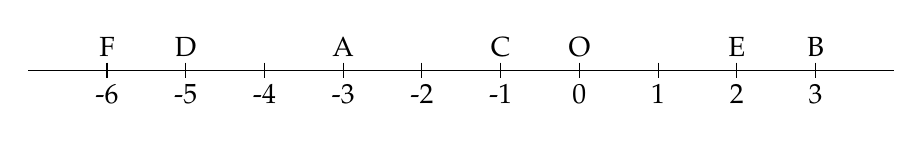
\begin{tikzpicture} 
\draw[-] (-7,0) -- (4,0); % Dessiner la droite 
\foreach \x in {-6,-5,-4,-3,-2,-1,0,1,2,3} % Dessiner les graduations
 \draw (\x,0.1) -- (\x,-0.1); 
 \node at (-6,0.3) {F}; 
 \node at (-5,0.3) {D}; 
 \node at (-3,0.3) {A};
 \node at (-1,0.3) {C}; 
 \node at (0,0.3) {O}; 
 \node at (2,0.3) {E}; 
 \node at (3,0.3) {B}; 
 \foreach \x in {-6,-5,-4,-3,-2,-1,0,1,2,3} % Étiqueter les graduations
 \node at (\x,-0.3) {\x};
 \end{tikzpicture}
\end{center}
\begin{enumerate}
	\item Déterminer les distances $OB$, $OC$, $OD$, $OE$ et $OF$.
\end{enumerate}
\end{Activite}

\begin{Definition}
Sur un axe normé, $x$ est l'abscisse d'un point $M$. \textcolor{red}{La valeur absolue} de $x$ est la distance entre l'origine du repère et le point $M$; on la note $|x|$.

En d'autre termes : $OM = |x|$ (où $O$ est l'origine du repère).
\end{Definition}
\begin{Exemple}
\begin{itemize}
	\item $|4| = 4$ et $|-3| = 3$ et $|-\dfrac{1}{2}| = \dfrac{1}{2}$.
	\item $|1 - \sqrt{2}| = \sqrt{2} - 1$.
\end{itemize}
\end{Exemple}

\begin{Proposition}
Soit $x$ un nombre réel. On a 
$|x| = 
\begin{cases} 
x \text{ si } x\geq 0 \\
-x \text{ si } x\leq 0
\end{cases}
$
\end{Proposition}

\begin{Definition}
Si $a$ et $b$ sont les abscisses respectives de deux points $A$ et $B$ sur un axe normé (droite graduée), alors la distance entre $a$ et $b$ est la distance $AB$ et on a : $AB = |a - b|$.
\end{Definition}

\begin{Proposition}
Soient $x$ et $y$ deux nombres réels. On a :
\begin{enumerate}
	\item $|x| \geq 0$
	\item $|-x| = |x|$
	\item $|x - y| = |y - x|$
	\item $|x^2| = |x|^2 = x^2$
	\item \textcolor{red}{$\sqrt{x^2} = |x|$}
	\item $|x\times y| = |x||y|$
	\item si $y\neq 0$, alors $\left|\dfrac{x}{y}\right| = \dfrac{|x|}{|y|}$
	\item \textcolor{red}{$|x + y| \leq |x| + |y|$}
	\item $|x - y| \geq |x| - |y|$
	\item \textcolor{red}{$|x| = |y|$ signifie que $x = y$ ou $x = - y$}.
\end{enumerate}
\end{Proposition}
&\\
\hline

\end{tabular}

\begin{tabular}{|>{\raggedright\arraybackslash}p{17cm}|>{\centering\arraybackslash}p{0.8cm}|}
\hline
\vspace{1mm}
\textcolor{red}{Remarque : }
$$
\begin{cases}
|x| = r \\
r > 0
\end{cases} \text{signifie que } (x = r \text{ ou } x = -r)
$$

\begin{Exemple}
\begin{itemize}
	\item $|x| = 4$ signifie que ($x = 5$ ou $x = -5$).
	\item $|x| = -4$ est impossible car $|x| \geq 0$ et $-4 < 0$.
	\item $|x - 1| = 3$ signifie que ($x - 1 = 3$ ou $x - 1 = -3$) c'est-à-dire ($x = 4$ ou $x  = -2$)
\end{itemize}
\end{Exemple}

\begin{Application}
Soit $x;y\in\mathbb{R}$ tel que $x\leq 2$ et $y\geq 3$. Simplifier le nombre $A$ tel que $A = \sqrt{(x - 2)^2} + \sqrt{(y - 3)^3}$.
\end{Application}

\begin{Proposition}
Soit $x;y\in\mathbb{R}$ et $r > 0$.
\begin{enumerate}
	\item $|x| \leq r$ signifie que $-r\leq x\leq r$
	\item $|x|\geq r$ signifie que $x\geq r$ ou $x\leq -r$.
\end{enumerate}
\end{Proposition}

\mysection{Intervalles}
\begin{Activite}


\end{Activite}


&\\
\hline

\end{tabular}





























\end{document}